%%%%%%%%%%%%%%%%%%%%%%%%%%%%%%%%%%%%%%%%%%%%%%%%%%%%%%%%%%%%%%%%%%%%%%%%
%                                                                      %
%     File: Thesis_Introduction.tex                                    %
%     Tex Master: Thesis.tex                                           %
%                                                                      %
%     Author: Rui Santiago                         			   %
%     Last modified : 2 Junho 2015                         		   %
%                                                                      %
%%%%%%%%%%%%%%%%%%%%%%%%%%%%%%%%%%%%%%%%%%%%%%%%%%%%%%%%%%%%%%%%%%%%%%%%

\chapter{Introdu\c{c}\~ao}
\label{chapter:introducao}

%O sistema num chip em inglês System On Chip \acrlong{soc} é um chip integrado que tem integrado todas as funcionalidades de computador ou de um sistema electrónico, num único chip. Um \acrshort{soc} é constituído tipicamente por vários elementos interligados entre si por um barramento. Os elementos podem ser separados por grupos conformes os seus principais funcionalidades, os principais grupos são os seguintes: processamento, memoria, fontes de \textcolor[rgb]{1,0,0}{timing}, periféricos, interfaces externas, interfaces analógicas e gestores de energia. Na figura \ref{figures:ARM} pode se um exemplo de um diagrama de blocos de um \acrshort{soc}, onde se pode o barramento ligação dos elementos.





A computação reconfigurável (CR) tem tido um grande foco na investigação na última década. As máquinas reconfiguráveis mudam dinamicamente a sua arquitectura de acordo com as instruções executadas.
Foi demonstrado que as CRs podem ter acelerações de grande magnitude em aplicações como processamento de sinal. Visto que o ramo das telecomunicações usa muitos sistemas de processamento de sinal, a importância dos CRs é enorme.

O Versat é um sistema que usa uma arquitectura reconfigurável. O objectivo principal do Versat é configurar e correr o Data Engine um certo número de vezes até ser produzido um resultado esperado.
O Versat não está desenhado para um alto desempenho ao nível da execução de instruções. O controlador tem o mínimo de instruções possível e serve essencialmente para controlar a execução do Data Engine.

O Versat estará ligado a um sistema mestre, sendo o próprio um sistema escravo. A interface de controlo é usada para efectuar as leituras e escritas necessárias entre mestre e escravo.

O Data Engine é onde os cálculos de alto desempenho são executados. Os dados de entrada estão organizados em vectores colocados em memória RAM de porto duplo, sendo que cada um dos portos tem um gerador de endereços.

O problema deste tipo de sistemas é o desenvolvimento de um compilador adequado. 
Ainda não existe um compilador eficiente para este tipo de máquinas.


%\begin{figure}[!htb]
 % \centering
 % \includegraphics[width=0.5\textwidth]{Figures/ARM_SOC.png}
 % \caption[Diagrama de blocos de um soc ARM ]{Diagrama de blocos de um soc ARM }
 % \label{figures:ARM}
  %http://en.wikipedia.org/wiki/System_on_a_chip
%\end{figure}

%Os \acrshort{soc} têm uma vasta possibilidade de utilização desde um simples relógio até no mais avançado tecnologicamente como no desenvolvimentos de módulos para satélites, passando pela industria automóvel e com o aparecimento do arduino cada vez mais os \acrshort{soc} são utilizados em projetos de pequena escala desenvolvidos em casa, porque veio permitir a pessoas de com pouco ou nenhum conhecimento na área programar e efectuar debug no seu projecto com o \acrshort{soc}. A sua utilização traz vantagens com preço baixo, baixo consumo de energia e dimensões pequenas, como tudo o que existe também tem desvantagens sendo neste caso o baixo poder de calculo comparado com um computador. %http://www.extremetech.com/computing/126235-soc-vs-cpu-the-battle-for-the-future-of-computing

%Com uma área tão vasta de aplicações não é de estranhar que existam várias empresas \textcolor[rgb]{1,0,0}{a muito tempo} e varias startup no mercado a desenvolver \acrshort{soc} para fins totalmente distintos, cada empresa optimizando o seu para que foi desenvolvido.



% --------------------------------------------------------------------- 


O objectivo deste trabalho é investigar o desenvolvimento de um compilador para o Versat. Deve ser levado em linha de conta que o Versat é um acelerador de {\it hardware} que usa uma arquitectura de computação reconfigurável.
Portanto é de esperar que a implementação do compilador seja muito diferente de uma implementação clássica. Serão escritos vários programas na linguagem desenvolvida para demonstrar o funcionamento correcto do compilador. Será também feito um estudo da arquitectura do Versat, com o objectivo de entender melhor o {\it hardware} e perceber a forma como fazer
o compilador o mais eficiente possível.

\cleardoublepage

%Uma startup no desenvolvimento de um projecto/produto necessita de um \acrshort{soc} para poder comercializar o seu produto. Na pesquisa do \acrshort{soc} ideal para o seu projecto encontram diferentes possibilidades, mas nenhuma preenchia todos os critérios pretendidos para o projecto. Como não foi encontrada uma solução ideal dos vários \acrshort{soc} disponíveis no mercado, a solução possível serias desenvolver o seu próprio \acrshort{soc} desenvolvido a medidas para o projecto.

% ----------------------------------------------------------------------
%\section{Motiva\c{c}\~ao}
%\label{section:motiva}

%\textcolor[rgb]{0,0,1}{desenvolver um sistema necessário para uma startup, o sistema vai ser desenvolvido a medida com o pretendido com a startup.}

%\section{Objectivos}
%\label{section:objectivo}

%A startup no desenvolvimento de um projeto/produto necessita de um \acrshort{soc}, como se pode ver na figura \ref{grafos:problema} que tem de ter a capacidade de processamento necessária para efetuar a descodificação e codificação de dados que irá receber e enviar. O \acrshort{soc} desenvolvido tem de permitir que sejas ligado mais dois modelos assíncronos permitindo a recolha de dados no local para posterior envio dos dados pelo modelo de comunicação. O produto é para ser usado em locais de difíceis acessos este terá de ter um baixo consumo, permitindo que a bateria funcione o maior tempo possível. Para alem do mencionado anteriormente também necessita de duas interfaces de comunicação \acrlong{uart} e \acrlong{gpio}. 

%\begin{figure}[!htb]
 % \centering
 % 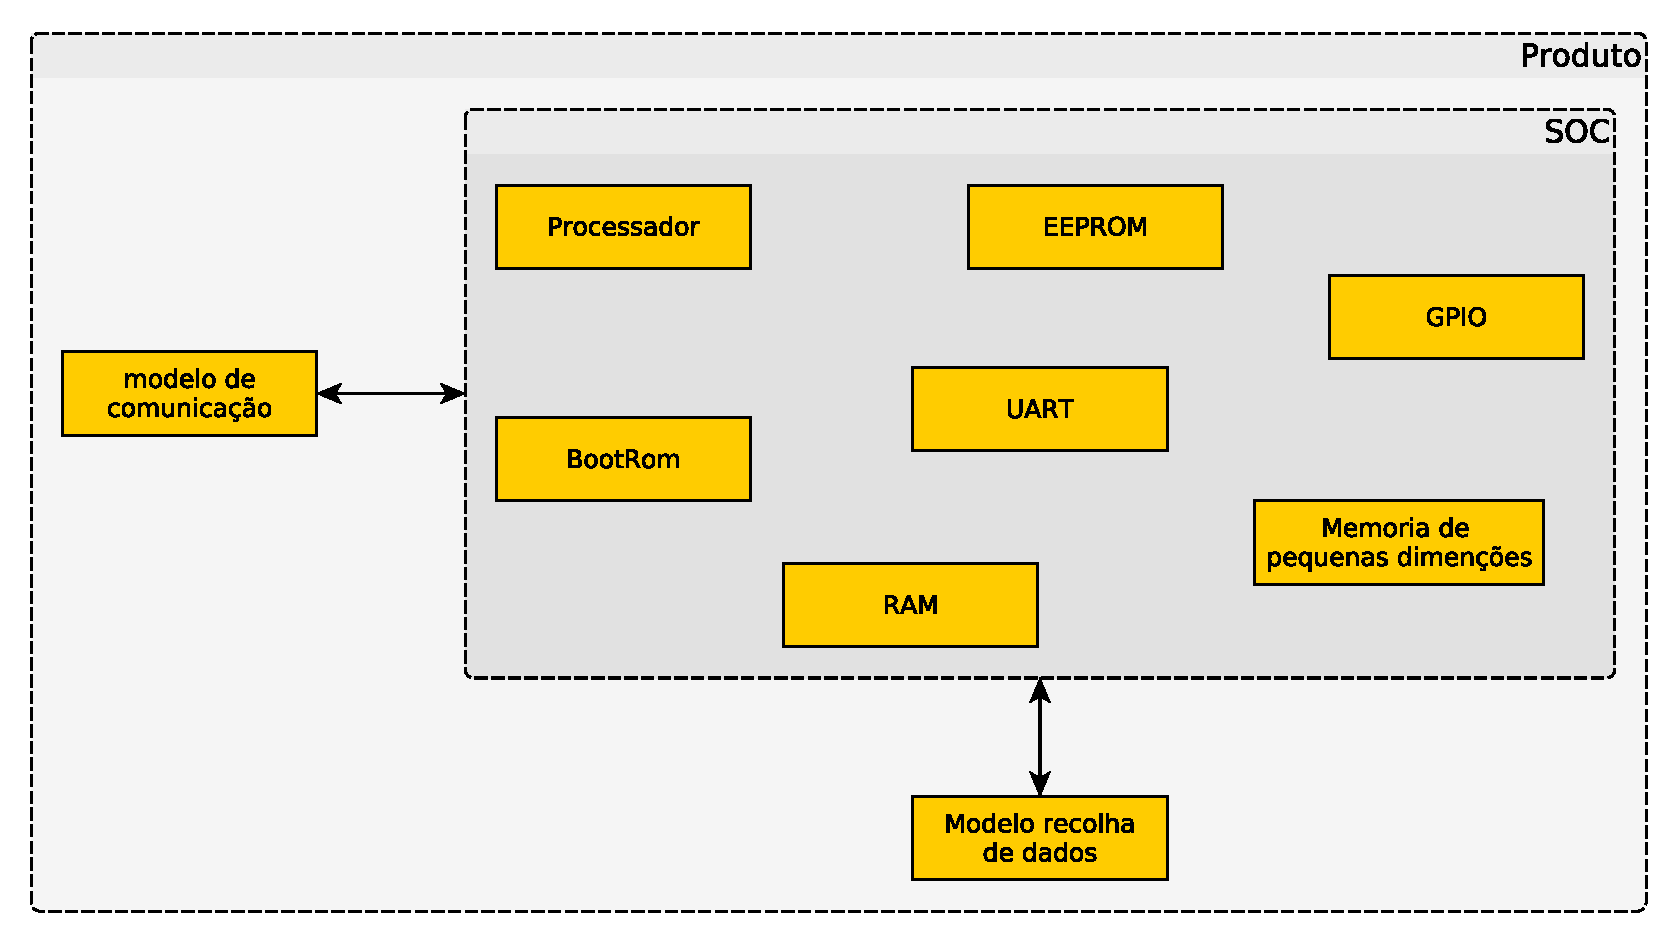
\includegraphics[width=0.5\textwidth]{grafos/problema.pdf}
 % \caption[SOC pretendido pela Startup]{SOC pretendido pela Startup}
 % \label{grafos:problema}
  %http://en.wikipedia.org/wiki/System_on_a_chip
%\end{figure}


%\section{Desafios}
%\label{section:desafio}


%Os principais desafios desta dissertação consiste no desenvolvimento de um sistema sintetizável que preencha todas as necessidades mencionadas pela startup.

%Desenvolver uma interface assíncrona necessária para a comunicação entre o \acrshort{soc} e os modelos de comunicação e de recolha de dados a ser desenvolvido pela startup.

%A criação de uma bootrom que carregua para a memoria principal o programa que se encontra na EEPROM. Ainda testa o mau funcionamento da EEPROM ou da memoria principal notificando o utilizador. 
